\begin{figure}[htbp]\centering
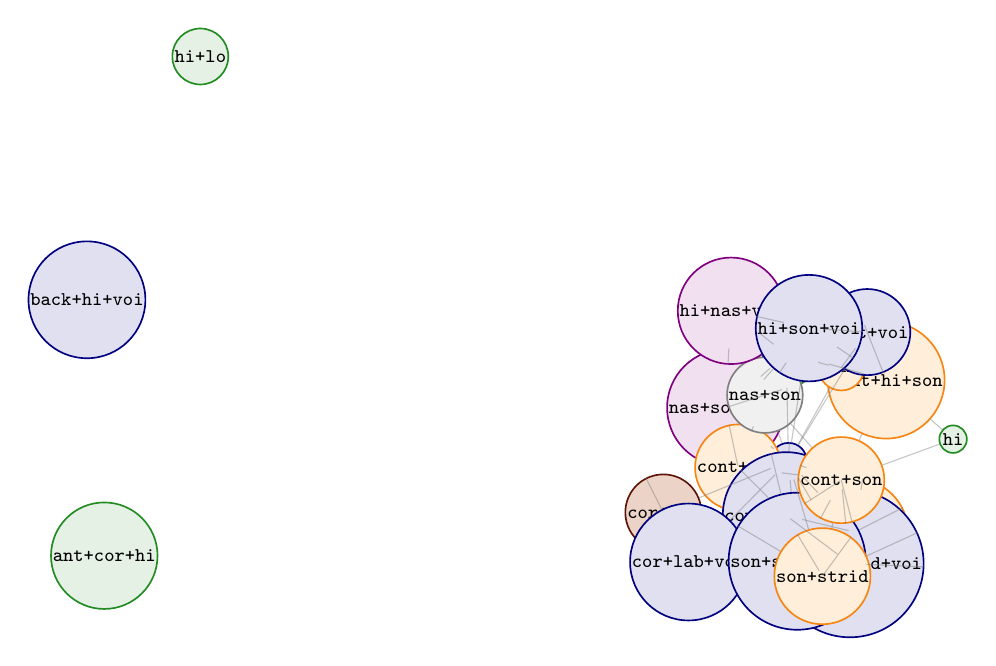
\begin{tikzpicture}[font=\scriptsize]
\node[circle,draw=ForestGreen,fill=ForestGreen!12,line width=0.6pt,inner sep=0.5pt,minimum size=0.40cm] (P0) at (-4.06,3.30) {\texttt{{hi+lo}}};
\node[circle,draw=Purple,fill=Purple!12,line width=0.6pt,inner sep=0.5pt,minimum size=0.39cm] (P1) at (2.61,-1.16) {\texttt{{nas+son+voi}}};
\node[circle,draw=NavyBlue,fill=NavyBlue!12,line width=0.6pt,inner sep=0.5pt,minimum size=0.37cm] (P2) at (3.41,-1.84) {\texttt{{voi}}};
\node[circle,draw=BurntOrange,fill=BurntOrange!12,line width=0.6pt,inner sep=0.5pt,minimum size=0.37cm] (P3) at (4.25,-2.74) {\texttt{{cont+strid}}};
\node[circle,draw=Sepia,fill=Sepia!12,line width=0.6pt,inner sep=0.5pt,minimum size=0.36cm] (P4) at (1.82,-2.49) {\texttt{{cor+lab}}};
\node[circle,draw=BurntOrange,fill=BurntOrange!12,line width=0.6pt,inner sep=0.5pt,minimum size=0.32cm] (P5) at (2.77,-1.92) {\texttt{{cont+nas}}};
\node[circle,draw=BurntOrange,fill=BurntOrange!12,line width=0.6pt,inner sep=0.5pt,minimum size=0.28cm] (P6) at (4.65,-0.81) {\texttt{{cont+hi+son}}};
\node[circle,draw=NavyBlue,fill=NavyBlue!12,line width=0.6pt,inner sep=0.5pt,minimum size=0.27cm] (P7) at (3.38,-2.53) {\texttt{{cont+son+voi}}};
\node[circle,draw=NavyBlue,fill=NavyBlue!12,line width=0.6pt,inner sep=0.5pt,minimum size=0.27cm] (P8) at (4.19,-3.14) {\texttt{{cont+strid+voi}}};
\node[circle,draw=ForestGreen,fill=ForestGreen!12,line width=0.6pt,inner sep=0.5pt,minimum size=0.26cm] (P9) at (3.38,-0.48) {\texttt{{hi+son}}};
\node[circle,draw=Gray,fill=Gray!12,line width=0.6pt,inner sep=0.5pt,minimum size=0.26cm] (P10) at (3.11,-1.00) {\texttt{{nas+son}}};
\node[circle,draw=BurntOrange,fill=BurntOrange!12,line width=0.6pt,inner sep=0.5pt,minimum size=0.25cm] (P11) at (4.08,-0.65) {\texttt{{cont}}};
\node[circle,draw=NavyBlue,fill=NavyBlue!12,line width=0.6pt,inner sep=0.5pt,minimum size=0.23cm] (P12) at (2.14,-3.12) {\texttt{{cor+lab+voi}}};
\node[circle,draw=NavyBlue,fill=NavyBlue!12,line width=0.6pt,inner sep=0.5pt,minimum size=0.23cm] (P13) at (3.52,-3.11) {\texttt{{son+strid+voi}}};
\node[circle,draw=BurntOrange,fill=BurntOrange!12,line width=0.6pt,inner sep=0.5pt,minimum size=0.18cm] (P14) at (4.08,-2.08) {\texttt{{cont+son}}};
\node[circle,draw=BurntOrange,fill=BurntOrange!12,line width=0.6pt,inner sep=0.5pt,minimum size=0.17cm] (P15) at (3.84,-3.30) {\texttt{{son+strid}}};
\node[circle,draw=NavyBlue,fill=NavyBlue!12,line width=0.6pt,inner sep=0.5pt,minimum size=0.17cm] (P16) at (4.41,-0.20) {\texttt{{cont+voi}}};
\node[circle,draw=NavyBlue,fill=NavyBlue!12,line width=0.6pt,inner sep=0.5pt,minimum size=0.16cm] (P17) at (-5.50,0.21) {\texttt{{back+hi+voi}}};
\node[circle,draw=ForestGreen,fill=ForestGreen!12,line width=0.6pt,inner sep=0.5pt,minimum size=0.15cm] (P18) at (-5.28,-3.04) {\texttt{{ant+cor+hi}}};
\node[circle,draw=Purple,fill=Purple!12,line width=0.6pt,inner sep=0.5pt,minimum size=0.15cm] (P19) at (2.68,0.07) {\texttt{{hi+nas+voi}}};
\node[circle,draw=NavyBlue,fill=NavyBlue!12,line width=0.6pt,inner sep=0.5pt,minimum size=0.15cm] (P20) at (3.67,-0.15) {\texttt{{hi+son+voi}}};
\node[circle,draw=ForestGreen,fill=ForestGreen!12,line width=0.6pt,inner sep=0.5pt,minimum size=0.14cm] (P21) at (5.50,-1.56) {\texttt{{hi}}};
\draw[gray,opacity=0.45,line width=0.4pt] (P1) -- (P2);
\draw[gray,opacity=0.45,line width=0.4pt] (P1) -- (P5);
\draw[gray,opacity=0.45,line width=0.4pt] (P1) -- (P7);
\draw[gray,opacity=0.45,line width=0.4pt] (P1) -- (P9);
\draw[gray,opacity=0.45,line width=0.4pt] (P1) -- (P10);
\draw[gray,opacity=0.45,line width=0.4pt] (P1) -- (P19);
\draw[gray,opacity=0.45,line width=0.4pt] (P2) -- (P3);
\draw[gray,opacity=0.45,line width=0.4pt] (P2) -- (P4);
\draw[gray,opacity=0.45,line width=0.4pt] (P2) -- (P7);
\draw[gray,opacity=0.45,line width=0.4pt] (P2) -- (P8);
\draw[gray,opacity=0.45,line width=0.4pt] (P2) -- (P9);
\draw[gray,opacity=0.45,line width=0.4pt] (P2) -- (P10);
\draw[gray,opacity=0.45,line width=0.4pt] (P2) -- (P11);
\draw[gray,opacity=0.45,line width=0.4pt] (P2) -- (P12);
\draw[gray,opacity=0.45,line width=0.4pt] (P2) -- (P13);
\draw[gray,opacity=0.45,line width=0.4pt] (P2) -- (P14);
\draw[gray,opacity=0.45,line width=0.4pt] (P2) -- (P15);
\draw[gray,opacity=0.45,line width=0.4pt] (P2) -- (P16);
\draw[gray,opacity=0.45,line width=0.4pt] (P2) -- (P20);
\draw[gray,opacity=0.45,line width=0.4pt] (P3) -- (P7);
\draw[gray,opacity=0.45,line width=0.4pt] (P3) -- (P8);
\draw[gray,opacity=0.45,line width=0.4pt] (P3) -- (P13);
\draw[gray,opacity=0.45,line width=0.4pt] (P3) -- (P14);
\draw[gray,opacity=0.45,line width=0.4pt] (P3) -- (P15);
\draw[gray,opacity=0.45,line width=0.4pt] (P4) -- (P12);
\draw[gray,opacity=0.45,line width=0.4pt] (P5) -- (P7);
\draw[gray,opacity=0.45,line width=0.4pt] (P5) -- (P10);
\draw[gray,opacity=0.45,line width=0.4pt] (P5) -- (P14);
\draw[gray,opacity=0.45,line width=0.4pt] (P6) -- (P9);
\draw[gray,opacity=0.45,line width=0.4pt] (P6) -- (P11);
\draw[gray,opacity=0.45,line width=0.4pt] (P6) -- (P14);
\draw[gray,opacity=0.45,line width=0.4pt] (P6) -- (P16);
\draw[gray,opacity=0.45,line width=0.4pt] (P6) -- (P20);
\draw[gray,opacity=0.45,line width=0.4pt] (P6) -- (P21);
\draw[gray,opacity=0.45,line width=0.4pt] (P7) -- (P8);
\draw[gray,opacity=0.45,line width=0.4pt] (P7) -- (P13);
\draw[gray,opacity=0.45,line width=0.4pt] (P7) -- (P14);
\draw[gray,opacity=0.45,line width=0.4pt] (P7) -- (P15);
\draw[gray,opacity=0.45,line width=0.4pt] (P8) -- (P13);
\draw[gray,opacity=0.45,line width=0.4pt] (P8) -- (P14);
\draw[gray,opacity=0.45,line width=0.4pt] (P8) -- (P15);
\draw[gray,opacity=0.45,line width=0.4pt] (P9) -- (P11);
\draw[gray,opacity=0.45,line width=0.4pt] (P9) -- (P19);
\draw[gray,opacity=0.45,line width=0.4pt] (P9) -- (P20);
\draw[gray,opacity=0.45,line width=0.4pt] (P10) -- (P14);
\draw[gray,opacity=0.45,line width=0.4pt] (P10) -- (P19);
\draw[gray,opacity=0.45,line width=0.4pt] (P10) -- (P20);
\draw[gray,opacity=0.45,line width=0.4pt] (P11) -- (P16);
\draw[gray,opacity=0.45,line width=0.4pt] (P13) -- (P14);
\draw[gray,opacity=0.45,line width=0.4pt] (P13) -- (P15);
\draw[gray,opacity=0.45,line width=0.4pt] (P14) -- (P15);
\draw[gray,opacity=0.45,line width=0.4pt] (P14) -- (P21);
\draw[gray,opacity=0.45,line width=0.4pt] (P16) -- (P20);
\draw[gray,opacity=0.45,line width=0.4pt] (P19) -- (P20);
\end{tikzpicture}
\caption{\textbf{Operator graph $G_O$ of Austronesian.} Nodes are operators (the 22 with highest support), sized by frequency and coloured by change type (\textcolor{NavyBlue}{voicing}, \textcolor{BurntOrange}{fricativization}, \textcolor{ForestGreen}{palatalization/height}, \textcolor{Sepia}{place}, \textcolor{Purple}{prenasalization}). An edge joins $u,v$ when their composition $u\oplus v$ is itself an operator of the repertoire --- so this is the graph of \emph{additive closure}. Dense connectivity is the visual face of the composition index $C(O)$.}
\end{figure}
